\documentclass[a4paper,oneside]{report}
\usepackage[fontsize=13pt]{scrextend}
\usepackage[utf8]{inputenc}
\usepackage[T5]{fontenc}
\usepackage[vietnamese]{babel}
\usepackage{times}
\usepackage[left=3.5cm,right=2.5cm,top=2cm,bottom=2cm,includehead,includefoot]{geometry}
\usepackage{setspace}
\setstretch{1.2}
\usepackage{indentfirst}
\setlength{\parskip}{4pt}
\usepackage{amsmath,amssymb}
\usepackage{graphicx,float,caption,subcaption}
\usepackage{booktabs,tabularx,longtable,multirow,array}
\usepackage[table]{xcolor}
\usepackage{enumitem}
\setlist{itemsep=1pt,parsep=0pt,topsep=3pt}
\emergencystretch=3em
\usepackage{listings}
\usepackage{tikz}
\usetikzlibrary{positioning,arrows.meta,fit}
\usepackage{fancyhdr}
\usepackage{titlesec,titletoc}
\usepackage[hidelinks]{hyperref}
\usepackage{xurl}
\usepackage[backend=biber,style=ieee]{biblatex}
\addbibresource{refs.bib}

\graphicspath{{figures/}}

% ---------- Tiêu đề chương / mục ----------
\titleformat{\chapter}[display]{\bfseries\centering\fontsize{16}{20}\selectfont}
  {CHƯƠNG \thechapter}{6pt}{\fontsize{16}{20}\selectfont\MakeUppercase}
\titlespacing*{\chapter}{0pt}{0pt}{18pt}
\titleformat{\section}{\bfseries\fontsize{14}{17}\selectfont}{\thesection}{0.6em}{}
\titleformat{\subsection}{\bfseries\itshape}{\thesubsection}{0.6em}{}
\titlecontents{chapter}[0cm]{\bfseries\vspace{0.3cm}}
  {\bfseries CHƯƠNG \thecontentslabel.\ }{}{\titlerule*[0.3pc]{.}\contentspage}
\titlecontents{section}[0cm]{\vspace{0.2cm}}{\thecontentslabel\ }{}{\titlerule*[0.3pc]{.}\contentspage}
\titlecontents{subsection}[1cm]{\vspace{0.1cm}}{\thecontentslabel\ }{}{\titlerule*[0.3pc]{.}\contentspage}

% ---------- Header / footer ----------
\pagestyle{fancy}
\fancyhf{}
\fancyhead[L]{\small Mạng thế hệ mới -- Đề tài 13}
\fancyhead[R]{\small\nouppercase{\leftmark}}
\renewcommand{\chaptermark}[1]{\markboth{\chaptername\ \thechapter}{}}
\fancyfoot[C]{\thepage}
\setlength{\headheight}{16pt}
\fancypagestyle{plain}{\fancyhf{}\fancyfoot[C]{\thepage}\renewcommand{\headrulewidth}{0pt}}

% ---------- Code listing ----------
\lstset{basicstyle=\ttfamily\footnotesize,breaklines=true,frame=single,
  columns=fullflexible,keepspaces=true,showstringspaces=false,
  backgroundcolor=\color{gray!8},numbers=left,numberstyle=\tiny\color{gray}}
\renewcommand{\lstlistingname}{Đoạn mã}

% ---------- Ghi chú việc cần làm (xóa trước khi nộp) ----------
\newcommand{\todo}[1]{\textcolor{red}{\textbf{[TODO]} #1}}

% ---------- Thông tin nhóm (sửa ở đây) ----------
\newcommand{\memberA}{Họ và tên thành viên 1}
\newcommand{\mshvA}{MSHV}
\newcommand{\memberB}{Họ và tên thành viên 2}
\newcommand{\mshvB}{MSHV}
\newcommand{\lecturer}{Tên giảng viên}
\newcommand{\classcode}{Mã lớp học phần}
\newcommand{\repourl}{\url{https://github.com/hieu2k2boss/Computer_Network_DeTai_13}}

\begin{document}
\begin{titlepage}
\begin{tikzpicture}[remember picture,overlay]
  \draw[line width=2pt] ([xshift=2.5cm,yshift=-1.5cm]current page.north west)
    rectangle ([xshift=-1.5cm,yshift=1.5cm]current page.south east);
  \draw[line width=0.6pt] ([xshift=2.65cm,yshift=-1.65cm]current page.north west)
    rectangle ([xshift=-1.65cm,yshift=1.65cm]current page.south east);
\end{tikzpicture}
\centering
{\bfseries\large ĐẠI HỌC BÁCH KHOA HÀ NỘI\\[2pt]
TRƯỜNG CÔNG NGHỆ THÔNG TIN VÀ TRUYỀN THÔNG\par}
\vspace{0.3cm}
\rule{0.5\linewidth}{0.8pt}
\vspace{1.6cm}

\IfFileExists{figures/logo-hust.png}{\includegraphics[height=3.2cm]{logo-hust}\par\vspace{1.2cm}}{\vspace{2.5cm}}

{\bfseries\fontsize{20}{24}\selectfont BÁO CÁO PROJECT GIỮA KỲ\par}
\vspace{0.4cm}
{\bfseries\large Môn học: MẠNG THẾ HỆ MỚI\par}
\vspace{1.2cm}

{\bfseries\large ĐỀ TÀI 13:\par}
\vspace{0.2cm}
{\bfseries\fontsize{17}{22}\selectfont TƯỜNG LỬA ỨNG DỤNG WEB VỚI\\
MODSECURITY/CORAZA VÀ OWASP CRS\par}
\vspace{0.3cm}
{\itshape Bảo vệ DVWA trước SQLi, XSS, LFI và Command Injection\par}

\vfill
\begin{tabular}{@{}ll@{}}
\textbf{Giảng viên hướng dẫn:} & \lecturer \\[4pt]
\textbf{Lớp học phần:} & \classcode \\[4pt]
\textbf{Nhóm thực hiện:} & 1. \memberA{} -- \mshvA \\
 & 2. \memberB{} -- \mshvB \\
\end{tabular}

\vspace{1.8cm}
{\bfseries Hà Nội, \today\par}
\end{titlepage}


\pagenumbering{roman}
\tableofcontents
\listoffigures
\listoftables
\chapter*{Danh mục từ viết tắt}
\addcontentsline{toc}{chapter}{Danh mục từ viết tắt}
\begin{tabularx}{\linewidth}{@{}lX@{}}
\toprule
\textbf{Viết tắt} & \textbf{Ý nghĩa} \\ \midrule
WAF & Web Application Firewall \\
CRS & OWASP Core Rule Set \\
DVWA & Damn Vulnerable Web Application \\
SQLi & SQL Injection \\
XSS & Cross-Site Scripting \\
LFI & Local File Inclusion \\
CMDi & Command Injection \\
PL & Paranoia Level \\
SecLang & ModSecurity Rule Language \\
TLS & Transport Layer Security \\
DDoS & Distributed Denial of Service \\
SIEM & Security Information and Event Management \\
\todo{bổ sung} & \\
\bottomrule
\end{tabularx}

\clearpage
\pagenumbering{arabic}
% Ngân sách: ~1.5 trang
\chapter{Giới thiệu}

\section{Bối cảnh}
\todo{Tấn công tầng ứng dụng web (OWASP Top 10~\cite{owasptop10}); vì sao tường lửa L3/L4 không đủ; vai trò của WAF.}

\section{Mục tiêu đề tài}
\begin{itemize}
  \item Tìm hiểu kiến trúc, nguyên lý hoạt động của ModSecurity/Coraza và OWASP CRS.
  \item So sánh với giải pháp truyền thống và thương mại.
  \item Triển khai lab bằng \texttt{docker-compose}, lặp lại được, lưu trên Git.
  \item Trình diễn bảo vệ DVWA trước SQLi, XSS, LFI, Command Injection.
  \item Đối chiếu yêu cầu TCVN 11930:2017 (cấp độ 2--3) với cấu hình và bằng chứng.
\end{itemize}

\section{Phạm vi và môi trường}
\todo{Lab cô lập (Docker network nội bộ), phiên bản phần mềm sử dụng, những gì nằm ngoài phạm vi.}

\section{Phân công công việc}
\begin{table}[H]
\centering
\caption{Phân công công việc trong nhóm}
\label{tab:phancong}
\begin{tabularx}{\linewidth}{@{}lX@{}}
\toprule
\textbf{Thành viên} & \textbf{Nhiệm vụ} \\ \midrule
\memberA & \todo{} \\
\memberB & \todo{} \\
\bottomrule
\end{tabularx}
\end{table}

% Yêu cầu 1 — Ngân sách: ~4 trang
\chapter{Kiến trúc và nguyên lý hoạt động}\label{chap:kientruc}

\section{Tổng quan về tường lửa ứng dụng web}
Tường lửa ứng dụng web (WAF) là thành phần kiểm tra nội dung giao dịch HTTP/HTTPS giữa người dùng và ứng dụng web, nhằm phát hiện và ngăn chặn các tấn công ở tầng ứng dụng như SQL Injection, Cross-Site Scripting hay Local File Inclusion~\cite{owasptop10}. Khác với tường lửa mạng chỉ xét địa chỉ IP, cổng và trạng thái kết nối, WAF phân tích cú pháp yêu cầu HTTP: đường dẫn, tham số, header, cookie và thân yêu cầu.

WAF có thể được triển khai theo ba mô hình: \textbf{reverse proxy} (WAF đứng trước ứng dụng, kết thúc TLS, kiểm tra rồi mới chuyển tiếp yêu cầu; đây là mô hình nhóm dùng trong lab), \textbf{nhúng} (chạy như một module trong máy chủ web Apache, Nginx) và \textbf{ngoài luồng} (nhận bản sao lưu lượng để phát hiện, không chặn trực tiếp).

Về chính sách, WAF có thể theo \textbf{mô hình âm} (negative security model: chặn những gì khớp mẫu tấn công đã biết) hoặc \textbf{mô hình dương} (positive security model: chỉ cho phép những gì đã được khai báo hợp lệ). Bộ OWASP CRS chủ yếu theo mô hình âm, với các luật tổng quát không gắn với một ứng dụng cụ thể.

\section{ModSecurity}
\subsection{Lịch sử và kiến trúc}
ModSecurity do Ivan Ristić phát triển từ năm 2002, ban đầu là một module của Apache HTTP Server~\cite{modsecbook}. Dự án sau đó được Breach Security rồi Trustwave SpiderLabs bảo trợ; năm 2024, khi Trustwave kết thúc hỗ trợ, dự án được chuyển giao cho OWASP~\cite{modsecurity}.

Có hai dòng phiên bản chính:
\begin{itemize}
  \item \textbf{ModSecurity v2:} gắn chặt với Apache, phụ thuộc vào cấu trúc dữ liệu nội bộ của Apache.
  \item \textbf{ModSecurity v3 (libmodsecurity):} viết lại bằng C++ thành một thư viện độc lập với máy chủ web. Máy chủ web tích hợp thông qua \emph{connector}, phổ biến nhất là \texttt{ModSecurity-nginx}. Mỗi yêu cầu HTTP được thư viện xử lý như một \emph{transaction}: connector chuyển từng phần dữ liệu (header, body) vào thư viện và nhận lại quyết định cho qua hay chặn.
\end{itemize}

ModSecurity bản thân chỉ là một \emph{bộ máy thực thi luật}; khả năng phát hiện tấn công đến từ bộ luật nạp vào, mà phổ biến nhất là OWASP CRS (mục~\ref{sec:crs}).

\subsection{Ngôn ngữ luật SecLang}
Luật và cấu hình ModSecurity được viết bằng ngôn ngữ SecLang. Một luật có cấu trúc:
\begin{center}
\texttt{SecRule BIẾN TOÁN\_TỬ "HÀNH\_ĐỘNG"}
\end{center}
\begin{itemize}
  \item \textbf{Biến} xác định phần dữ liệu cần kiểm tra, ví dụ \texttt{ARGS} (tham số), \texttt{REQUEST\_HEADERS}, \texttt{REQUEST\_URI}, \texttt{REQUEST\_BODY}, hay biến giao dịch \texttt{TX}.
  \item \textbf{Toán tử} xác định cách so khớp: \texttt{@rx} (biểu thức chính quy), \texttt{@pm} (khớp nhiều chuỗi), \texttt{@detectSQLi} và \texttt{@detectXSS} (dùng thư viện libinjection~\cite{libinjection} để phân tích cú pháp thay vì so khớp mẫu).
  \item \textbf{Hành động} gồm: định danh (\texttt{id}, \texttt{phase}, \texttt{msg}, \texttt{severity}, \texttt{tag}); biến đổi dữ liệu trước khi so khớp (\texttt{t:urlDecodeUni}, \texttt{t:lowercase}, \texttt{t:htmlEntityDecode}) để chống né tránh bằng mã hóa; hành động ngắt (\texttt{deny}, \texttt{block}, \texttt{pass}, \texttt{drop}); và gán biến (\texttt{setvar}).
\end{itemize}

\begin{lstlisting}[caption={Một luật SecLang phát hiện SQLi bằng libinjection},label={lst:seclang}]
SecRule ARGS "@detectSQLi" \
    "id:100001,phase:2,block,t:none,t:urlDecodeUni,\
    log,msg:'SQL Injection (libinjection)',severity:'CRITICAL',\
    setvar:'tx.inbound_anomaly_score_pl1=+%{tx.critical_anomaly_score}'"
\end{lstlisting}

Luật trong Đoạn mã~\ref{lst:seclang} kiểm tra mọi tham số ở pha 2, giải mã URL trước khi phân tích, và nếu phát hiện SQLi thì ghi log và cộng điểm bất thường thay vì chặn ngay. Cách cộng điểm này là nền tảng của cơ chế anomaly scoring trong CRS.

Bên cạnh luật, một số chỉ thị cấu hình quan trọng:
\begin{itemize}
  \item \texttt{SecRuleEngine On | Off | DetectionOnly}: bật chặn, tắt, hoặc chỉ phát hiện.
  \item \texttt{SecRequestBodyAccess} / \texttt{SecResponseBodyAccess}: cho phép kiểm tra thân yêu cầu / phản hồi.
  \item \texttt{SecAuditEngine}, \texttt{SecAuditLogParts}, \texttt{SecAuditLogFormat}: điều khiển nhật ký kiểm toán (audit log), có thể xuất dạng JSON để đưa vào hệ thống SIEM.
\end{itemize}

\subsection{Các pha xử lý giao dịch HTTP}
ModSecurity chia mỗi giao dịch thành năm pha (Hình~\ref{fig:phases}); mỗi luật được gán vào một pha qua hành động \texttt{phase}:
\begin{enumerate}
  \item \textbf{Request headers:} ngay sau khi nhận xong header yêu cầu. Phù hợp với luật về phương thức, URI, header.
  \item \textbf{Request body:} sau khi đọc thân yêu cầu (form, JSON, multipart). Phần lớn luật phát hiện tấn công chạy ở pha này vì đã có đủ tham số.
  \item \textbf{Response headers:} trước khi gửi header phản hồi về người dùng.
  \item \textbf{Response body:} kiểm tra nội dung phản hồi, ví dụ phát hiện rò rỉ thông báo lỗi SQL hay mã nguồn.
  \item \textbf{Logging:} sau khi giao dịch kết thúc; chỉ ghi log, không thể chặn.
\end{enumerate}

\begin{figure}[!htb]
\centering
\begin{tikzpicture}[
  box/.style={draw,rounded corners,minimum width=2.3cm,minimum height=9mm,font=\footnotesize,align=center},
  end/.style={draw,minimum width=1.7cm,minimum height=9mm,font=\footnotesize,align=center,fill=gray!15},
  lbl/.style={font=\scriptsize}]
  \node[end] (cli) at (0,0) {Người\\dùng};
  \node[box] (p1) at (3,0) {Pha 1\\Request headers};
  \node[box] (p2) at (6.2,0) {Pha 2\\Request body};
  \node[end] (app) at (9.4,0) {Ứng dụng\\web};
  \node[box] (p3) at (6.2,-2) {Pha 3\\Response headers};
  \node[box] (p4) at (3,-2) {Pha 4\\Response body};
  \node[draw,rounded corners,fill=gray!8,font=\footnotesize] (p5) at (4.6,-3.4) {Pha 5 -- Logging: ghi audit log sau khi giao dịch kết thúc};
  \draw[-Stealth] (cli) -- (p1);
  \draw[-Stealth] (p1) -- (p2);
  \draw[-Stealth] (p2) -- node[lbl,above]{cho qua} (app);
  \draw[-Stealth] (app) |- (p3);
  \draw[-Stealth] (p3) -- (p4);
  \draw[-Stealth] (p4) -| (cli);
  \draw[-Stealth,dashed,red!70!black] (p2.north) -- ++(0,0.6) -| (cli.north);
  \node[lbl,text=red!70!black] at (3,0.85) {điểm inbound $\geq$ ngưỡng: chặn, trả 403};
\end{tikzpicture}
\caption{Các pha xử lý của ModSecurity/Coraza khi đặt làm reverse proxy}
\label{fig:phases}
\end{figure}

\section{Coraza}
OWASP Coraza là một WAF mã nguồn mở viết bằng Go, cài đặt lại bộ máy SecLang của ModSecurity~\cite{coraza}. Coraza dùng cùng cú pháp luật và chạy được nguyên bộ OWASP CRS, nên chính sách viết cho ModSecurity có thể chuyển sang Coraza mà gần như không phải sửa. Khác biệt chính:
\begin{itemize}
  \item \textbf{Ngôn ngữ và an toàn bộ nhớ:} Go loại bỏ nhiều lớp lỗi bộ nhớ thường gặp ở mã C/C++.
  \item \textbf{Tích hợp:} Coraza là thư viện Go, nhúng trực tiếp vào ứng dụng Go hoặc dùng qua các tích hợp với Caddy, Envoy/Istio (proxy-wasm), HAProxy (SPOA), thay vì connector cho Nginx/Apache.
  \item \textbf{Tình trạng dự án:} Coraza được phát triển tích cực trong hệ sinh thái cloud-native, trong khi ModSecurity v3 hiện chủ yếu được sửa lỗi và vá bảo mật.
\end{itemize}
Vì hai phần mềm dùng chung SecLang và CRS, các nguyên lý trình bày ở mục này và mục~\ref{sec:crs} áp dụng cho cả hai. Lab của nhóm dùng ModSecurity v3 trên Nginx.

\section{OWASP Core Rule Set}\label{sec:crs}
\subsection{Cấu trúc bộ luật}
OWASP Core Rule Set (CRS) là bộ luật phát hiện tấn công tổng quát dùng cho ModSecurity, Coraza và nhiều WAF tương thích~\cite{crs}. Các luật được chia thành tệp theo nhóm tấn công, đánh số theo dải ID; Bảng~\ref{tab:crsfiles} liệt kê các nhóm liên quan đến kịch bản demo. Cấu hình chung (ngưỡng điểm, paranoia level) nằm trong \texttt{crs-setup.conf}.

\begin{table}[!htb]
\centering
\caption{Một số nhóm luật CRS liên quan đến đề tài}
\label{tab:crsfiles}
\small
\begin{tabularx}{\linewidth}{@{}llX@{}}
\toprule
\textbf{Dải ID} & \textbf{Tệp luật} & \textbf{Nội dung} \\ \midrule
920xxx & REQUEST-920-PROTOCOL-ENFORCEMENT & Kiểm tra tuân thủ giao thức HTTP \\
930xxx & REQUEST-930-APPLICATION-ATTACK-LFI & Path traversal, truy cập tệp hệ thống \\
932xxx & REQUEST-932-APPLICATION-ATTACK-RCE & Chèn lệnh hệ điều hành \\
941xxx & REQUEST-941-APPLICATION-ATTACK-XSS & Cross-Site Scripting \\
942xxx & REQUEST-942-APPLICATION-ATTACK-SQLI & SQL Injection \\
949xxx & REQUEST-949-BLOCKING-EVALUATION & So sánh điểm inbound với ngưỡng \\
959xxx & RESPONSE-959-BLOCKING-EVALUATION & So sánh điểm outbound với ngưỡng \\
\bottomrule
\end{tabularx}
\end{table}

\subsection{Cơ chế chấm điểm bất thường (anomaly scoring)}
CRS mặc định hoạt động theo cơ chế chấm điểm. Mỗi luật khi khớp không chặn ngay mà cộng vào điểm bất thường của giao dịch một giá trị theo mức nghiêm trọng: CRITICAL cộng 5, ERROR cộng 4, WARNING cộng 3, NOTICE cộng 2. Cuối pha 2, luật trong tệp 949 so tổng điểm inbound với ngưỡng (mặc định 5); nếu đạt hoặc vượt ngưỡng, yêu cầu bị chặn và audit log ghi luật 949110 kèm danh sách các luật đã góp điểm. Tương tự, cuối pha 4 tệp 959 đánh giá điểm outbound (ngưỡng mặc định 4).


Cơ chế này có hai ưu điểm. Thứ nhất, một yêu cầu chỉ khớp một luật nhẹ (ví dụ NOTICE) sẽ không bị chặn, giảm chặn nhầm. Thứ hai, quản trị viên có thể điều chỉnh độ nhạy bằng một tham số duy nhất là ngưỡng, và đọc được trong log vì sao một yêu cầu bị chặn.

\subsection{Paranoia level}
Mỗi luật CRS được gắn một mức paranoia (PL) từ 1 đến 4:
\begin{itemize}
  \item \textbf{PL1} (mặc định): luật chắc chắn, rất ít chặn nhầm; phù hợp hầu hết ứng dụng.
  \item \textbf{PL2}: thêm luật bắt các biến thể tấn công khó hơn; bắt đầu cần tinh chỉnh.
  \item \textbf{PL3, PL4}: luật rất chặt (ví dụ hạn chế ký tự đặc biệt), phát hiện tốt hơn nhưng chặn nhầm nhiều, đòi hỏi viết luật loại trừ cho từng ứng dụng.
\end{itemize}
CRS~4 dùng biến \texttt{tx.blocking\_paranoia\_level} để chọn mức luật được phép góp điểm chặn, và \texttt{tx.detection\_paranoia\_level} để chạy thêm các luật ở mức cao hơn nhưng chỉ ghi log. Nhờ đó có thể quan sát tác động của một mức cao hơn trên lưu lượng thật trước khi bật chặn.

\subsection{Chế độ DetectionOnly và Blocking}
Chỉ thị \texttt{SecRuleEngine} quyết định WAF có thực thi hành động chặn hay không:
\begin{itemize}
  \item \textbf{DetectionOnly:} mọi luật vẫn được đánh giá và ghi log, nhưng hành động ngắt (\texttt{deny}, \texttt{block}) không được thực thi. Quy trình khuyến nghị là chạy chế độ này với PL1 khi mới triển khai, thu thập các trường hợp chặn nhầm và viết luật loại trừ, rồi mới chuyển sang Blocking.
  \item \textbf{On (Blocking):} yêu cầu vượt ngưỡng bị chặn, mặc định trả về mã 403.
\end{itemize}

% Yêu cầu 2 — Ngân sách: ~2 trang
\chapter{So sánh với giải pháp truyền thống và thương mại}\label{chap:sosanh}

\section{So sánh với tường lửa mạng truyền thống}
Tường lửa mạng truyền thống (iptables/nftables, OPNsense, các thiết bị stateful firewall) ra quyết định dựa trên thông tin tầng 3--4: địa chỉ IP nguồn/đích, giao thức, cổng và trạng thái kết nối. Với một ứng dụng web công khai, tường lửa buộc phải mở cổng 80/443 cho mọi người dùng, nên một yêu cầu tấn công như
\begin{center}
\texttt{GET /vulnerabilities/sqli/?id=1' OR '1'='1}
\end{center}
về mặt tầng 3--4 hoàn toàn giống một yêu cầu hợp lệ và được cho qua. Hơn nữa, khi lưu lượng được mã hóa TLS, tường lửa mạng không nhìn thấy nội dung HTTP.

WAF bổ sung cho tường lửa mạng chứ không thay thế: WAF kết thúc TLS, phân tích cú pháp HTTP, chuẩn hóa dữ liệu (giải mã URL, HTML entity) rồi mới so khớp luật, nên phát hiện được tấn công nằm trong tham số. Ngược lại, WAF không lọc các giao thức khác ngoài HTTP và không thay được vai trò phân vùng mạng của tường lửa. IDS/IPS mạng như Suricata cũng có luật cho tấn công web nhưng làm việc trên gói tin, khó xử lý lưu lượng đã mã hóa.

\section{So sánh với WAF thương mại}
Nhóm chọn ba đại diện cho ba hướng triển khai thương mại: \textbf{F5 BIG-IP Advanced WAF} (trước đây là BIG-IP ASM), thiết bị phần cứng hoặc máy ảo đặt tại trung tâm dữ liệu của tổ chức~\cite{f5waf}; \textbf{Cloudflare WAF}, dịch vụ đám mây mà lưu lượng đi qua mạng biên của Cloudflare nhờ trỏ DNS~\cite{cloudflarewaf}; và \textbf{AWS WAF}, dịch vụ gắn với CloudFront, Application Load Balancer, API Gateway của AWS~\cite{awswaf}. Bảng~\ref{tab:sosanh} tóm tắt so sánh.

\begin{table}[!htb]
\centering
\caption{So sánh ModSecurity/Coraza + CRS với một số WAF thương mại}
\label{tab:sosanh}
\footnotesize
\renewcommand{\arraystretch}{1.12}
\begin{tabularx}{\linewidth}{@{}>{\raggedright\arraybackslash}p{2.0cm}*{4}{>{\raggedright\arraybackslash}X}@{}}
\toprule
\textbf{Tiêu chí} & \textbf{ModSecurity / Coraza + CRS} & \textbf{F5 Advanced WAF} & \textbf{Cloudflare WAF} & \textbf{AWS WAF} \\ \midrule
Giấy phép, chi phí & Nguồn mở (Apache 2.0), miễn phí; chi phí là công vận hành & Giấy phép thương mại, chi phí cao & Thuê bao theo gói; gói miễn phí có bộ luật cơ bản & Trả theo số web ACL, số luật và số yêu cầu \\
Triển khai & Tự cài trên máy chủ, container, Kubernetes & Thiết bị hoặc máy ảo tại chỗ & Đám mây, qua DNS & Chỉ trên tài nguyên AWS \\
Bộ luật & CRS cộng đồng, có thể xem và sửa từng luật & Chữ ký của F5 và chính sách tự học & Bộ luật do Cloudflare quản lý, có phiên bản dựa trên CRS & AWS Managed Rules và luật của bên thứ ba \\
Mô hình bảo mật & Chủ yếu mô hình âm & Cả âm và dương (học chính sách từ lưu lượng) & Chủ yếu mô hình âm & Chủ yếu mô hình âm \\
Chống bot, DDoS tầng 7 & Không có sẵn; cần kết hợp công cụ khác & Có & Có, là thế mạnh & Có, một số tính năng tính phí riêng \\
Quản trị, giám sát & Tệp cấu hình và log; cần tự xây giao diện, SIEM & Giao diện quản trị đầy đủ & Bảng điều khiển web, API & Bảng điều khiển AWS, CloudWatch \\
Dữ liệu và TLS & Ở trong hạ tầng của tổ chức & Ở trong hạ tầng của tổ chức & Nhà cung cấp kết thúc TLS và thấy nội dung & Ở trong hạ tầng AWS \\
\bottomrule
\end{tabularx}
\end{table}

\section{Nhận xét}
Điểm mạnh của ModSecurity/Coraza + CRS là chi phí bản quyền bằng không, tính minh bạch (đọc được từng luật và biết chính xác vì sao một yêu cầu bị chặn) và khả năng triển khai ở bất kỳ đâu, kể cả trong mạng nội bộ không kết nối Internet, giữ dữ liệu và khóa TLS trong hạ tầng của tổ chức.

Đổi lại, tổ chức phải tự chịu chi phí vận hành: tinh chỉnh luật loại trừ, cập nhật CRS, xây dựng giám sát và cảnh báo. Các giải pháp thương mại bù vào phần này bằng giao diện quản trị, bộ luật được nhà cung cấp cập nhật liên tục, đội ngũ hỗ trợ, và các tính năng mà giải pháp nguồn mở không có sẵn như chống bot, chống DDoS tầng 7. Tóm lại, WAF đám mây hợp với ứng dụng công khai cần chịu tải lớn, F5 hợp với tổ chức lớn cần mô hình bảo mật dương, còn ModSecurity/Coraza hợp khi ngân sách hạn chế hoặc cần kiểm soát hoàn toàn chính sách.

% Ngân sách: ~3 trang
\chapter{Triển khai hệ thống}\label{chap:trienkhai}

\section{Mô hình lab}
Lab gồm ba container trên một máy (Hình~\ref{fig:topology}), chia vào hai mạng Docker:
\begin{itemize}
  \item \textbf{\texttt{edge}} (mạng bridge thường): WAF và DVWA. Máy chủ chỉ công bố hai cổng trên \texttt{127.0.0.1}: \texttt{8080} vào WAF và \texttt{8081} vào thẳng DVWA. Đường \texttt{8081} không qua WAF, dùng làm đối chứng để chứng minh lỗ hổng có thật.
  \item \textbf{\texttt{backend}} (\texttt{internal: true}): WAF, DVWA và MariaDB. Docker không tạo đường ra ngoài cho mạng này nên CSDL không gửi được gói tin ra Internet.
\end{itemize}
Địa chỉ IP do Docker cấp động; các container gọi nhau bằng tên dịch vụ (\texttt{dvwa}, \texttt{db}) nên cấu hình không phụ thuộc IP.

\begin{figure}[!htb]
\centering
\begin{tikzpicture}[box/.style={draw,rounded corners,minimum width=2.4cm,minimum height=10mm,font=\footnotesize,align=center}]
  \node[box] (att) at (-0.8,0) {Máy chủ lab\\(trình duyệt, curl,\\\texttt{attack.sh})};
  \node[box,fill=orange!15] (waf) at (5.4,0) {WAF\\Nginx + ModSecurity\\+ OWASP CRS};
  \node[box] (dvwa) at (9.4,0) {DVWA\\(Apache + PHP)};
  \node[box] (db) at (9.4,-2) {MariaDB};
  \node[box] (log) at (-0.8,-2) {Audit log JSON\\(\texttt{docker logs})};
  \draw[-Stealth] (att) -- node[pos=0.35,above,font=\scriptsize]{127.0.0.1:8080} (waf);
  \draw[-Stealth] (waf) -- node[above,font=\scriptsize]{:80} (dvwa);
  \draw[-Stealth,dashed] (att.north) -- ++(0,0.9) -| node[pos=0.25,above,font=\scriptsize]{127.0.0.1:8081 (đối chứng, không WAF)} (dvwa.north);
  \draw[-Stealth] (dvwa) -- (db);
  \draw[-Stealth,dashed] (waf.south west) -- (log.north east);
  \node[draw,dotted,inner sep=2mm,fit=(waf)(dvwa),label={[font=\scriptsize,anchor=north west]south west:\texttt{edge}}] {};
  \node[draw,densely dashed,inner sep=7mm,fit=(waf)(dvwa)(db),label={[font=\scriptsize]below:\texttt{backend} (internal, không ra Internet)}] {};
\end{tikzpicture}
\caption{Mô hình lab triển khai}
\label{fig:topology}
\end{figure}

\section{Thành phần và phiên bản}
Mọi image được ghim theo digest SHA-256 trong \texttt{docker-compose.yml}, nên chạy lại ở thời điểm khác vẫn cho ra đúng các phiên bản ở Bảng~\ref{tab:components} (đọc từ trường \texttt{producer} của audit log).

\begin{table}[!htb]
\centering
\caption{Thành phần phần mềm}
\label{tab:components}
\footnotesize
\begin{tabularx}{\linewidth}{@{}lllX@{}}
\toprule
\textbf{Thành phần} & \textbf{Image} & \textbf{Phiên bản} & \textbf{Vai trò} \\ \midrule
WAF & \texttt{owasp/modsecurity-crs:nginx} & ModSecurity v3.0.17, & Reverse proxy, lọc HTTP \\
 & & ModSecurity-nginx v1.0.4, & \\
 & & OWASP CRS 4.30.0 & \\
DVWA & \texttt{ghcr.io/digininja/dvwa} & ghim theo digest & Ứng dụng web có lỗ hổng \\
CSDL & \texttt{mariadb:11.4} & 11.4 & Dữ liệu DVWA \\
\bottomrule
\end{tabularx}
\end{table}

\section{Script cài đặt}
Toàn bộ cấu hình lab nằm tại kho mã \repourl{} (thư mục \texttt{lab/}). Đoạn mã~\ref{lst:compose} là phần khai báo dịch vụ WAF.

\begin{lstlisting}[caption={Trích đoạn \texttt{lab/docker-compose.yml} (dịch vụ WAF)},label={lst:compose}]
waf:
  image: owasp/modsecurity-crs:nginx@sha256:c95914e1...
  environment:
    BACKEND: http://dvwa:80
    MODSEC_RULE_ENGINE: ${MODSEC_RULE_ENGINE:-On}   # On | DetectionOnly | Off
    BLOCKING_PARANOIA: ${BLOCKING_PARANOIA:-1}      # 1..4
    ANOMALY_INBOUND: ${ANOMALY_INBOUND:-5}
    ANOMALY_OUTBOUND: ${ANOMALY_OUTBOUND:-4}
    MODSEC_AUDIT_ENGINE: RelevantOnly
    MODSEC_AUDIT_LOG_FORMAT: JSON
    MODSEC_AUDIT_LOG: /dev/stdout
  volumes:   # luat loai tru, nap sau CRS
    - ${EXCLUSION_FILE:-./rules/none.conf}:/etc/.../RESPONSE-999-EXCLUSION-RULES-AFTER-CRS.conf:ro
  ports: ["127.0.0.1:${WAF_PORT:-8080}:8080"]
  networks: [edge, backend]
\end{lstlisting}

Image của CRS sinh tệp cấu hình ModSecurity từ biến môi trường lúc khởi động, nên mọi thí nghiệm chỉ cần đổi biến rồi chạy \texttt{docker compose up -d waf}:
\begin{itemize}
  \item \path{MODSEC_RULE_ENGINE}, \path{BLOCKING_PARANOIA}, \path{ANOMALY_INBOUND/OUTBOUND}: gán \texttt{SecRuleEngine}, \texttt{tx.blocking\_paranoia\_level} và hai ngưỡng điểm (mặc định 5 và 4) của CRS~4.
  \item \texttt{MODSEC\_AUDIT\_*}: ghi audit log dạng JSON ra stdout của container, đọc bằng \texttt{docker compose logs waf} và dễ chuyển tiếp sang SIEM.
  \item \texttt{EXCLUSION\_FILE}: tệp luật loại trừ được gắn vào vị trí \texttt{RESPONSE-999-EXCLUSION-RULES-AFTER-CRS.conf}, tức nạp sau toàn bộ CRS (mục~\ref{sec:tinhchinh}).
\end{itemize}

\section{Cấu hình WAF}
Đoạn mã~\ref{lst:modsecconf} là các chỉ thị có hiệu lực, đọc trong container khi chạy cấu hình mặc định.

\begin{lstlisting}[caption={Cấu hình ModSecurity và CRS có hiệu lực trong container WAF},label={lst:modsecconf}]
SecRuleEngine On
SecRequestBodyAccess on
SecResponseBodyAccess on
SecAuditEngine RelevantOnly
SecAuditLogRelevantStatus "^(?:5|4(?!04))"
SecAuditLogParts ABIJDEFHZ
SecAuditLogFormat JSON
SecAuditLog /dev/stdout
# crs-setup.conf
setvar:tx.blocking_paranoia_level=1
setvar:tx.inbound_anomaly_score_threshold=5
setvar:tx.outbound_anomaly_score_threshold=4
\end{lstlisting}

Bật \texttt{SecResponseBodyAccess} cho phép các luật pha 4 (nhóm 950--959) phát hiện rò rỉ thông tin trong phản hồi. \texttt{SecAuditEngine RelevantOnly} kết hợp \texttt{SecAuditLogRelevantStatus} chỉ ghi các giao dịch có luật khớp hoặc trả mã 5xx/4xx (trừ 404), tránh log phình to vì lưu lượng bình thường. Kịch bản chính dùng PL1 không có luật loại trừ; PL2--PL4 và tệp \texttt{lab/rules/dvwa-exclusions.conf} chỉ dùng trong thí nghiệm ở Chương~\ref{chap:hanche}.

\section{Kiểm tra hoạt động}
Đoạn mã~\ref{lst:check} là kết quả khởi động lab và kiểm tra nhanh. Yêu cầu hợp lệ đi qua WAF bình thường, yêu cầu mang payload SQLi bị chặn, cổng WAF không truy cập được từ địa chỉ LAN của máy, và container CSDL không ra được Internet.

\begin{lstlisting}[language=bash,caption={Khởi động và kiểm tra lab},label={lst:check}]
$ cd lab && docker compose up -d && docker compose ps
db     Up (healthy)
dvwa   Up            127.0.0.1:8081->80/tcp
waf    Up (healthy)  127.0.0.1:8080->8080/tcp
$ curl -s -o /dev/null -w '%{http_code}\n' http://127.0.0.1:8080/login.php
200
$ curl -s -o /dev/null -w '%{http_code}\n' \
    "http://127.0.0.1:8080/login.php?id=1%27%20OR%20%271%27%3D%271"
403
$ curl -m 3 http://<IP-LAN-cua-may>:8080/     # tu dia chi LAN
curl: (7) Failed to connect                    # cong chi bind 127.0.0.1
$ docker compose exec db bash -c '</dev/tcp/1.1.1.1/53'
bash: connect: Network is unreachable          # mang backend internal
\end{lstlisting}

% Yêu cầu 4 — Ngân sách: ~4 trang
\chapter{Kịch bản trình diễn và kết quả}\label{chap:demo}

\section{Phương pháp đánh giá}
Mỗi payload được gửi theo hai đường tới cùng một DVWA (mức bảo mật \textit{low}): trực tiếp qua cổng 8081 (không WAF) và qua WAF ở cổng 8080. Hai đường dùng chung CSDL, chỉ khác nhau ở việc có đi qua ModSecurity hay không, nên mọi khác biệt về kết quả là do WAF. Với mỗi lần gửi, nhóm ghi nhận ba thông tin: mã trạng thái HTTP, việc khai thác có thành công hay không (dựa vào dấu hiệu trong nội dung trả về, ví dụ dòng \texttt{root:x:0:0} của \texttt{/etc/passwd}), và các luật CRS đã khớp trong audit log. Một yêu cầu hợp lệ (\texttt{id=1}) cũng được gửi kèm để kiểm tra WAF không chặn nhầm.

Các bước thực hiện lab như sau:
\begin{enumerate}
\item Khởi động lab: \texttt{cd lab \&\& docker compose up -d}, chờ MariaDB sẵn sàng.
\item Tạo CSDL DVWA qua \texttt{/setup.php} (nút \textit{Create / Reset Database}).
\item Đăng nhập \texttt{admin}/\texttt{password} trên cả hai cổng.
\item Gửi từng payload ở mục~\ref{sec:sqli}--\ref{sec:conlai} theo đường trực tiếp, rồi qua WAF.
\item Đọc audit log bằng \texttt{docker compose logs waf}, lọc theo từng yêu cầu.
\item Đổi \texttt{MODSEC\_RULE\_ENGINE=DetectionOnly}, khởi động lại riêng container \texttt{waf} và lặp lại bước 4--5.
\end{enumerate}
Bước 2--5 được tự động hóa bằng \texttt{lab/scripts/attack.sh}. Script gắn header \texttt{X-Demo-Case} vào mỗi yêu cầu để ghép kết quả với bản ghi audit log tương ứng, rồi lưu toàn bộ bằng chứng (nội dung từng phản hồi, \texttt{audit.json}, \texttt{summary.txt}) vào \texttt{lab/evidence/}.

\section{Kịch bản chi tiết: SQL Injection}\label{sec:sqli}
Trang \textit{SQL Injection} của DVWA ghép tham số \texttt{id} thẳng vào câu truy vấn. Nhóm gửi payload kinh điển \texttt{id=1' OR '1'='1}, làm điều kiện \texttt{WHERE} luôn đúng. Khi gửi trực tiếp, DVWA trả về toàn bộ năm người dùng trong bảng \texttt{users} thay vì một (Hình~\ref{fig:sqli}a). Khi gửi qua WAF, yêu cầu bị chặn với mã 403 trước khi tới DVWA (Hình~\ref{fig:sqli}b).

\begin{figure}[!htb]
\centering
\begin{subfigure}[b]{0.5\linewidth}
\centering
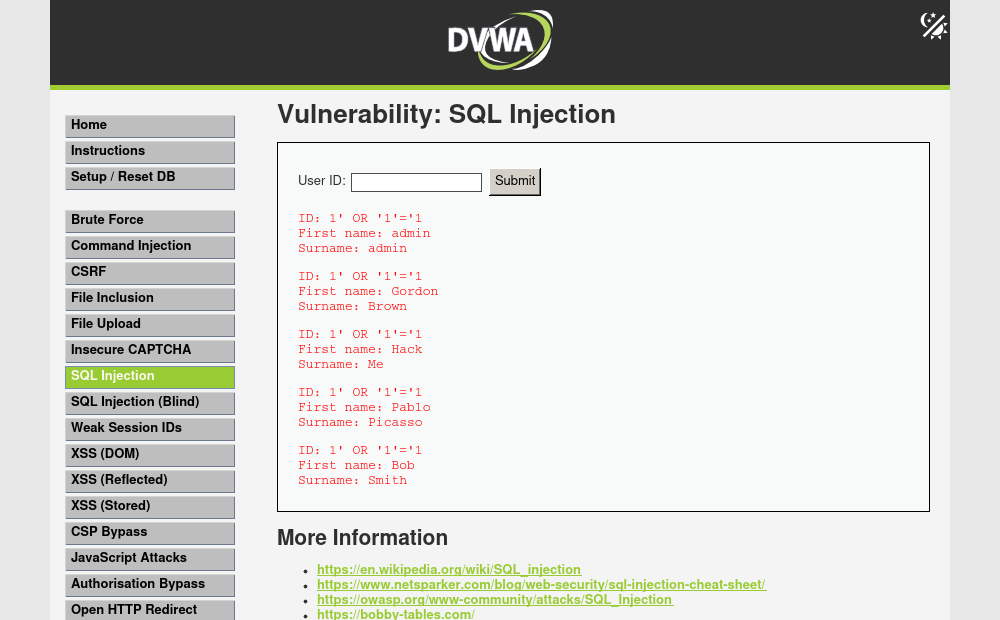
\includegraphics[width=\linewidth,trim=260 150 60 95,clip]{sqli-direct}
\caption{Không WAF: lộ toàn bộ bảng \texttt{users}}
\end{subfigure}\hfill
\begin{subfigure}[b]{0.36\linewidth}
\centering
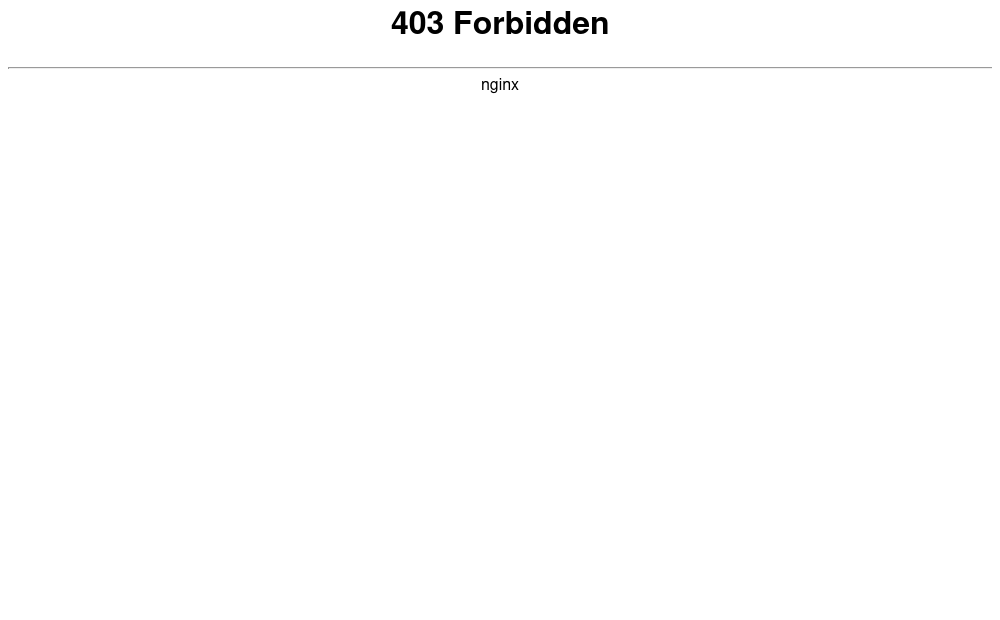
\includegraphics[width=\linewidth,trim=250 500 250 0,clip]{sqli-waf}
\caption{Qua WAF: 403 Forbidden}
\end{subfigure}
\caption{Cùng payload SQLi gửi tới DVWA trực tiếp và qua WAF}
\label{fig:sqli}
\end{figure}

Listing~\ref{lst:audit-sqli} là bản ghi audit log của yêu cầu bị chặn (đã lược bớt các trường không liên quan).

\begin{lstlisting}[caption={Audit log JSON của yêu cầu SQLi bị chặn (rút gọn)},label={lst:audit-sqli}]
{"transaction": {
  "request":  {"uri": "/vulnerabilities/sqli/?id=1%27%20OR%20%271%27%3D%271..."},
  "response": {"http_code": 403},
  "messages": [
    {"message": "SQL Injection Attack Detected via libinjection",
     "details": {"ruleId": "942100", "severity": "2",
       "data": "Matched Data: s&sos found within ARGS:id: 1' OR '1'='1"}},
    {"message": "Inbound Anomaly Score Exceeded (Total Score: 5)",
     "details": {"ruleId": "949110", "severity": "0"}}]}}
\end{lstlisting}

Bản ghi cho thấy đúng cơ chế chấm điểm bất thường đã trình bày ở Chương~\ref{chap:kientruc}. Trong pha 2, luật 942100 gọi libinjection trên tham số \texttt{ARGS:id}; libinjection nhận ra chuỗi token \texttt{s\&sos} (chuỗi -- toán tử -- chuỗi -- toán tử -- chuỗi) đặc trưng cho SQLi. Luật có mức CRITICAL (severity 2) nên cộng 5 điểm. Cuối pha 2, luật 949110 so tổng điểm 5 với ngưỡng \texttt{inbound\_anomaly\_score\_threshold} = 5, thấy đạt ngưỡng nên trả 403. Chỉ một luật khớp cũng đủ chặn, vì ngưỡng mặc định ở PL1 bằng đúng điểm của một luật CRITICAL.

\section{Các kịch bản còn lại}\label{sec:conlai}
\paragraph{Reflected XSS.} Payload \texttt{<script>alert(1)</script>} trong tham số \texttt{name} của trang \textit{XSS (Reflected)}. Không có WAF, DVWA chèn nguyên đoạn script vào trang và trình duyệt thực thi. Qua WAF, bốn luật khớp: 941100 (libinjection phát hiện XSS), 941110 (thẻ \texttt{<script>}), 941160 (chèn HTML) và 941390 (gọi hàm JavaScript \texttt{alert(}), tổng 20 điểm.

\paragraph{Local File Inclusion.} Tham số \texttt{page} của trang \textit{File Inclusion} được \texttt{include} trực tiếp, nên \texttt{?page=../../../../../../etc/passwd} in ra nội dung tệp mật khẩu hệ thống. Qua WAF, các luật 930100/930110 (chuỗi \texttt{../} trên tham số và trên URI thô), 930120 (truy cập tệp hệ điều hành nhạy cảm) và 932160 cùng khớp, tổng 30 điểm.

\paragraph{Command Injection.} Trang \textit{Command Injection} chạy lệnh \texttt{ping} với tham số \texttt{ip}. Payload \texttt{127.0.0.1;cat /etc/passwd} (gửi bằng POST) nối thêm lệnh thứ hai sau dấu \texttt{;}. Qua WAF, luật 930120 và 932160 (phát hiện mã shell Unix) khớp, tổng 10 điểm. Cả hai luật đều bắt chuỗi \texttt{etc/passwd}, không phải dấu \texttt{;} hay lệnh \texttt{cat}. Mục~\ref{sec:pl} cho thấy hệ quả: đổi sang một lệnh ngắn khác thì kết quả thay đổi.

\section{Tổng hợp kết quả}
Bảng~\ref{tab:ketqua} tổng hợp kết quả chạy \texttt{attack.sh} ở chế độ Blocking với cấu hình mặc định (PL1, ngưỡng vào 5, ngưỡng ra 4). Cả bốn loại tấn công đều khai thác được khi không có WAF và đều bị chặn khi đi qua WAF; yêu cầu hợp lệ không bị chặn nhầm. Mọi yêu cầu bị chặn đều kèm luật 949110, không liệt kê lại trong bảng.

\begin{table}[!htb]
\centering
\caption{Kết quả chặn tấn công (Blocking, PL1)}
\label{tab:ketqua}
\footnotesize
\begin{tabularx}{\linewidth}{@{}l>{\raggedright\arraybackslash}p{4.6cm}>{\raggedright\arraybackslash}p{1.9cm}ccX@{}}
\toprule
\textbf{Loại} & \textbf{Payload} & \textbf{Không WAF} & \textbf{Có WAF} & \textbf{Điểm} & \textbf{Luật khớp} \\ \midrule
Hợp lệ & \path{id=1} & 200 & 200 & 0 & -- \\
SQLi & \path{id=1' OR '1'='1} & 200, lộ dữ liệu & 403 & 5 & 942100 \\
XSS & \path{<script>alert(1)</script>} & 200, chạy script & 403 & 20 & 941100, 941110, 941160, 941390 \\
LFI & \path{page=../../../../../../etc/passwd} & 200, đọc tệp & 403 & 30 & 930100, 930110, 930120, 932160 \\
CMDi & \path{ip=127.0.0.1;cat /etc/passwd} & 200, chạy lệnh & 403 & 10 & 930120, 932160 \\
\bottomrule
\end{tabularx}
\end{table}

\section{So sánh DetectionOnly và Blocking}
Khi chuyển \texttt{MODSEC\_RULE\_ENGINE} sang \texttt{DetectionOnly} và chạy lại cùng bộ payload, mọi yêu cầu qua WAF đều trả 200 và khai thác thành công như khi không có WAF. Tuy vậy, audit log vẫn ghi đủ các luật khớp và điểm như ở Bảng~\ref{tab:ketqua}, kể cả luật 949110: ModSecurity vẫn đánh giá yêu cầu nhưng không thực hiện hành động chặn.

Kịch bản LFI còn ghi thêm hai luật đầu ra: 953100 (\textit{PHP Information Leakage}, phát hiện thông báo lỗi PHP trong nội dung phản hồi, mức ERROR, 4 điểm) và 959100 (vượt ngưỡng điểm đầu ra 4). Ở chế độ Blocking không thấy hai luật này vì yêu cầu đã bị chặn ở pha 2, phản hồi không bao giờ được sinh ra. Như vậy pha 4 kiểm tra được cả dữ liệu trả về, và DetectionOnly phù hợp để chạy thử trước khi bật chặn, nhằm thống kê luật nào chặn nhầm lưu lượng thật.

\section{Ảnh hưởng của paranoia level}\label{sec:pl}
Nhóm thử thêm payload \texttt{ip=127.0.0.1;id} trên trang \textit{Command Injection}, tức chạy lệnh \texttt{id} thay cho \texttt{cat /etc/passwd}, ở các mức paranoia khác nhau (biến \texttt{BLOCKING\_PARANOIA}), đồng thời gửi lại yêu cầu hợp lệ \texttt{sqli/?id=1}:
\begin{itemize}
\item PL1 và PL2: payload trả 200, lệnh chạy được (trang hiện \texttt{uid=33(www-data)}), không luật nào khớp; yêu cầu hợp lệ trả 200.
\item PL3: payload bị chặn (403, luật 932350); nhưng yêu cầu hợp lệ \texttt{?id=1} cũng bị chặn bởi chính luật này.
\end{itemize}

Với yêu cầu hợp lệ, audit log ghi \texttt{Matched Data: id found within ARGS\_NAMES:id}: luật so khớp cả \emph{tên} tham số, và tên \texttt{id} trùng với tên một lệnh Unix. Đây là ví dụ cụ thể về sự đánh đổi giữa bỏ sót và chặn nhầm khi tăng paranoia level. Cách khắc phục bằng luật loại trừ được trình bày ở mục~\ref{sec:tinhchinh}.

% Yêu cầu 6 (bắt buộc nhóm B) — Ngân sách: ~2.5 trang
\chapter{Đối chiếu với TCVN 11930:2017}\label{chap:tcvn}

\section{Giới thiệu tiêu chuẩn}
TCVN 11930:2017~\cite{tcvn11930} quy định yêu cầu cơ bản về an toàn hệ thống thông tin theo năm cấp độ (Điều 5 đến Điều 9). Mỗi cấp độ gồm yêu cầu quản lý và yêu cầu kỹ thuật; yêu cầu kỹ thuật chia thành bốn nhóm: an toàn mạng, máy chủ, ứng dụng và dữ liệu. Nhóm đối chiếu với yêu cầu kỹ thuật cấp độ 3 (Điều 7) và ghi kèm điều khoản tương ứng của cấp độ 2 (Điều 6) khi có. Đáng chú ý, mục 7.2.3.6~c nêu đích danh các dạng tấn công mà đề tài trình diễn: \textit{``Có phương án bảo vệ ứng dụng chống lại những dạng tấn công phổ biến: SQL Injection, OS command injection, RFI, LFI, Xpath injection, XSS, CSRF''}.

\section{Bảng đối chiếu}
Cột \textit{Mức}: \textbf{Đ} đáp ứng, \textbf{MP} một phần, \textbf{K} không đáp ứng (cần thành phần khác).

\begin{footnotesize}
\renewcommand{\arraystretch}{1.1}
\begin{longtable}{@{}>{\raggedright\arraybackslash}p{3.7cm}>{\raggedright\arraybackslash}p{5.6cm}>{\raggedright\arraybackslash}p{3.6cm}c@{}}
\caption{Đối chiếu điều khoản TCVN 11930:2017 -- cấu hình -- bằng chứng}\label{tab:tcvn}\\
\toprule
\textbf{Điều khoản} & \textbf{Cấu hình đáp ứng} & \textbf{Bằng chứng} & \textbf{Mức} \\ \midrule
\endfirsthead
\toprule
\textbf{Điều khoản} & \textbf{Cấu hình đáp ứng} & \textbf{Bằng chứng} & \textbf{Mức} \\ \midrule
\endhead
\bottomrule
\endfoot
7.2.3.6~c -- Chống SQLi, OS command injection, LFI, RFI, XSS, \ldots
& \texttt{SecRuleEngine On}; CRS 4.30.0 nhóm 930 (LFI), 931 (RFI), 932 (RCE), 941 (XSS), 942 (SQLi); PL1, ngưỡng vào 5
& Bảng~\ref{tab:ketqua}, Hình~\ref{fig:sqli}
& MP \\
7.2.3.6~a (6.2.3.4) -- Kiểm tra dữ liệu đầu vào
& Pha 1--2 kiểm tra header, tham số, thân yêu cầu; nhóm 920 kiểm tra tuân thủ HTTP
& Listing~\ref{lst:audit-sqli}
& MP \\
7.2.3.6~b, d -- Kiểm tra dữ liệu đầu ra; kiểm soát thông báo lỗi
& \texttt{SecResponseBodyAccess On}; pha 4 với nhóm 950--959 (953100: lộ lỗi PHP), ngưỡng ra 4; trang 403 không lộ thông tin ứng dụng
& Mục 5.5 (luật 953100, 959100)
& MP \\
7.2.1.5~a (6.2.1.5~a) -- Phòng chống xâm nhập
& WAF dạng reverse proxy trước máy chủ web, chế độ Blocking
& Chương~\ref{chap:demo}
& Đ \\
7.2.1.5~b (6.2.1.5~b) -- Cập nhật dấu hiệu tấn công
& CRS cố định theo digest image; cập nhật bằng cách đổi digest rồi chạy lại bộ kiểm thử
& \texttt{docker-compose.yml}
& MP \\
7.2.1.5~c -- Năng lực đáp ứng quy mô
& Đo thông lượng ở PL1, PL4 (\texttt{scripts/bench.sh})
& Bảng~\ref{tab:bench}
& MP \\
7.2.1.4~a -- Nhật ký: thời gian, IP/cổng, hành động, cảnh báo
& Audit log JSON: \texttt{time\_stamp}, \texttt{client\_ip}, \texttt{client\_port}, \texttt{http\_code}, các luật khớp
& Listing~\ref{lst:audit-sqli}
& Đ \\
7.2.3.3~a (6.2.3.3~a) -- Nhật ký truy cập ứng dụng, lỗi
& Access log, error log của nginx; audit log
& \texttt{docker compose logs waf}
& MP \\
7.2.1.4~c, đ; 7.2.3.3~b, c -- Lưu tập trung, tối thiểu 03 tháng
& Chưa có: lab chỉ ghi log ra stdout của container
& --
& K \\
7.2.1.1~b -- Kiểm soát truy cập giữa các vùng; an toàn máy chủ CSDL
& Mạng \texttt{edge} và \texttt{backend} (\texttt{internal: true}); CSDL chỉ ở \texttt{backend}, không ra Internet
& \texttt{docker-compose.yml}
& MP \\
7.2.1.2~đ, 7.2.3.2~đ -- Giới hạn kết nối đồng thời
& CRS không có chức năng này
& --
& K \\
\end{longtable}
\end{footnotesize}

\section{Nhận xét mức độ đáp ứng}
WAF đáp ứng trực tiếp nhất mục 7.2.3.6~c: bốn trong bảy dạng tấn công được nêu (SQLi, OS command injection, LFI, XSS) đã bị chặn trong Chương~\ref{chap:demo}; CRS có nhóm 931 cho RFI nhưng nhóm chưa kiểm thử. Mức đánh giá chỉ là \textit{một phần} vì: CSRF không phát hiện được bằng chữ ký mà phải sửa ở ứng dụng (token chống CSRF); XPath injection chưa kiểm thử; và PL1 vẫn bỏ sót command injection dạng ngắn (mục~\ref{sec:hanche}). Các mục 7.2.3.6~a, b, d cũng chỉ đáp ứng một phần vì WAF là lớp bảo vệ chung, không thay được việc ứng dụng tự kiểm tra dữ liệu theo nghiệp vụ.

Audit log đã có đủ các trường mục 7.2.1.4~a yêu cầu, nhưng cấp độ 3 còn đòi lưu tập trung và giữ tối thiểu 03 tháng; lab mới ghi ra stdout nên cần đẩy log về một SIEM như Wazuh hoặc Loki/Grafana (yêu cầu 7 của đề tài). Giới hạn kết nối đồng thời nằm ngoài khả năng của CRS, có thể bổ sung bằng \texttt{limit\_conn}/\texttt{limit\_req} của nginx. Như vậy, một mình ModSecurity + CRS không đủ cho cấp độ 3.

% Yêu cầu 5 — Ngân sách: ~3.5 trang
\chapter{Hạn chế và kết luận}\label{chap:hanche}

\section{Hạn chế của phần mềm}\label{sec:hanche}
Ngoài kịch bản chính ở Chương~\ref{chap:demo}, nhóm chạy thêm ba thí nghiệm trên cùng lab để lượng hóa các hạn chế: 15 biến thể payload (\texttt{lab/cases/bypass.txt}), 10 thao tác hợp lệ trên DVWA ở bốn mức paranoia (\texttt{lab/cases/benign.txt}), và đo hiệu năng (\texttt{lab/scripts/bench.sh}). Kết quả lưu trong \texttt{lab/evidence/}.

\subsection{Bỏ sót tấn công và vượt qua bằng biến thể payload}
Bảng~\ref{tab:bypass} cho thấy CRS ở PL1 chống tốt các kỹ thuật né tránh kinh điển cho SQLi, XSS và LFI. Đổi hoa thường, chèn chú thích \texttt{/**/}, thay \texttt{OR} bằng \texttt{||} hay mã hóa URL hai lần đều không qua được, vì trước khi so khớp, ModSecurity giải mã và chuẩn hóa dữ liệu (\texttt{t:urlDecodeUni}, \texttt{t:lowercase}, \ldots), còn libinjection phân tích theo token chứ không theo chuỗi cố định.

\begin{table}[!htb]
\centering
\caption{Kết quả 15 biến thể payload (số bị chặn / số biến thể)}
\label{tab:bypass}
\footnotesize
\begin{tabularx}{\linewidth}{@{}l>{\raggedright\arraybackslash}Xccl@{}}
\toprule
\textbf{Loại} & \textbf{Biến thể} & \textbf{PL1} & \textbf{PL3} & \textbf{Luật chính} \\ \midrule
SQLi & \path{/**/} thay khoảng trắng; \path{||} thay \texttt{OR}; \texttt{LIKE}; mã hóa URL 2 lần & 4/4 & 4/4 & 942100 \\
XSS & \path{<ScRiPt>}; \path{<svg/onload=...>}; \path{<img onerror=...>} & 3/3 & 3/3 & 941100--941390 \\
LFI & \path{/etc/passwd}, \path{/etc/hosts} (không có \texttt{../}); \path{php://filter} & 3/3 & 3/3 & 930120, 933140 \\
CMDi & \path{;cat ../../config/config.inc.php} & 1/1 & 1/1 & 930100--930120 \\
CMDi & \path{;id}, \path{|id}, xuống dòng + \texttt{id}, \path{;pwd} & \textbf{0/4} & 4/4 & 932350 (PL3) \\
\bottomrule
\end{tabularx}
\end{table}

Điểm yếu nằm ở payload ngắn, ít đặc trưng. Bốn biến thể command injection dùng lệnh hai, ba ký tự (\texttt{id}, \texttt{pwd}) lọt qua PL1 hoàn toàn và chạy được trên máy chủ, vì các luật bắt lệnh Unix không kèm đối số chỉ có từ PL3. Đây là hệ quả của triết lý thiết kế CRS: PL1 ưu tiên ít chặn nhầm, chấp nhận bỏ sót. Kẻ tấn công có thể dùng chính các lệnh ngắn này để dò môi trường trước khi viết payload dài hơn.

Ngoài ra, WAF dựa trên chữ ký không hiểu ngữ nghĩa ứng dụng. Nó không bảo vệ được lỗi logic nghiệp vụ, lỗi phân quyền (IDOR) hay CSRF (yêu cầu giả mạo trông hoàn toàn hợp lệ), và không chống dò mật khẩu nếu không kết hợp giới hạn tốc độ. Với lưu lượng HTTPS, WAF chỉ có tác dụng khi được đặt ở điểm kết thúc TLS.

\subsection{Chặn nhầm yêu cầu hợp lệ}
Bảng~\ref{tab:fp} là số thao tác hợp lệ (trong 10 thao tác) bị chặn ở từng mức. Ở PL1 không có chặn nhầm. Từ PL2, một lời nhắn sổ lưu bút có các từ \textit{select \ldots\ from \ldots\ drop} bị luật 942200/942260 coi là SQLi. Ở PL3, luật 932350 chặn mọi yêu cầu có tham số tên \texttt{id} như đã phân tích ở mục~\ref{sec:pl}. Ở PL4, luật 920273 chỉ chấp nhận một tập ký tự rất hẹp nên chặn cả tên \textit{Nguyen Van An} (vì dấu cách), \textit{O'Brien} và một địa chỉ email.

\begin{table}[!htb]
\centering
\caption{Số thao tác hợp lệ bị chặn nhầm (trên 10 thao tác)}
\label{tab:fp}
\footnotesize
\begin{tabularx}{\linewidth}{@{}lcc>{\raggedright\arraybackslash}X@{}}
\toprule
\textbf{Mức} & \textbf{Không loại trừ} & \textbf{Có 1 luật loại trừ} & \textbf{Luật gây chặn nhầm} \\ \midrule
PL1 & 0 & 0 & -- \\
PL2 & 1 & 1 & 942200, 942260 (sổ lưu bút) \\
PL3 & 3 & 1 & 932350 (tham số \texttt{id}); 942200, 942260 \\
PL4 & 6 & 4 & thêm 920273 (ký tự ngoài tập rất hẹp), 942432 \\
\bottomrule
\end{tabularx}
\end{table}

Kết hợp hai bảng cho thấy sự đánh đổi trực tiếp: muốn chặn được \texttt{;id} phải lên PL3, nhưng khi đó 3/10 thao tác hợp lệ bị chặn.

\subsection{Chi phí tinh chỉnh luật}\label{sec:tinhchinh}
Cách khắc phục chặn nhầm là viết luật loại trừ (rule exclusion). Listing~\ref{lst:excl} là luật nhóm viết cho DVWA, nạp sau CRS qua biến \texttt{EXCLUSION\_FILE}. Luật chỉ bỏ \emph{tên} tham số \texttt{id} khỏi danh sách biến mà 932350 kiểm tra; \emph{giá trị} các tham số vẫn được kiểm tra như cũ.

\begin{lstlisting}[caption={Luật loại trừ cho DVWA (\texttt{lab/rules/dvwa-exclusions.conf})},label={lst:excl}]
SecRuleUpdateTargetById 932350 "!ARGS_NAMES:id"
\end{lstlisting}

Với một dòng này, PL3 cho qua yêu cầu \texttt{?id=1} nhưng vẫn chặn đủ 15/15 biến thể ở Bảng~\ref{tab:bypass} và cả bốn kịch bản ở Chương~\ref{chap:demo}. Tuy vậy, PL3 vẫn chặn nhầm sổ lưu bút và PL4 còn bốn trường hợp; mỗi trường hợp cần một luật loại trừ riêng, viết đủ hẹp để không mở lỗ hổng mới. Quy trình hợp lý là chạy DetectionOnly với lưu lượng thật, đọc audit log tìm luật khớp với yêu cầu hợp lệ, viết luật loại trừ hẹp nhất có thể, rồi chạy lại bộ tấn công. Việc này phải làm lại cho từng ứng dụng và sau mỗi lần nâng cấp CRS; CRS chỉ có sẵn gói loại trừ cho một số ứng dụng phổ biến như WordPress, Drupal, Nextcloud.

\subsection{Chi phí hiệu năng}
Bảng~\ref{tab:bench} là kết quả đo bằng ApacheBench với 10 kết nối đồng thời, mỗi cấu hình 3000 yêu cầu, chạy 5 vòng xen kẽ và lấy trung vị. Yêu cầu đo là một tệp CSS tĩnh kèm ba tham số: WAF vẫn kiểm tra đầy đủ, còn thời gian xử lý của backend gần bằng 0, nên chênh lệch phản ánh chi phí của WAF.

\begin{table}[!htb]
\centering
\caption{Hiệu năng theo cấu hình (trung vị 5 vòng, \texttt{ab -n 3000 -c 10})}
\label{tab:bench}
\footnotesize
\begin{tabular}{@{}lrrr@{}}
\toprule
\textbf{Cấu hình} & \textbf{Yêu cầu/giây} & \textbf{Thời gian TB (ms)} & \textbf{Thêm so với \texttt{Off} (ms)} \\ \midrule
DVWA trực tiếp & 14\,555 & 0,69 & -- \\
Nginx, ModSecurity tắt (\texttt{Off}) & 5\,944 & 1,68 & 0 \\
ModSecurity + CRS, PL1 & 2\,221 & 4,50 & 2,82 \\
ModSecurity + CRS, PL4 & 1\,667 & 6,00 & 4,32 \\
\bottomrule
\end{tabular}
\end{table}

Mỗi yêu cầu tốn thêm khoảng 2,8~ms ở PL1 và 4,3~ms ở PL4 so với chỉ dùng nginx làm proxy; thông lượng giảm khoảng 63\% và 72\%. Với một trang động mất hàng chục ms để sinh ra, độ trễ thêm này là nhỏ, nhưng dưới tải cao WAF tiêu tốn CPU đáng kể và phải được tính khi định cỡ hệ thống. Số liệu đo trên một máy 8 nhân chạy chung các dịch vụ khác, chỉ có ý nghĩa so sánh tương đối.

\section{Hướng phát triển}
\begin{itemize}
  \item \textbf{Tập trung nhật ký:} đẩy audit log JSON về Wazuh hoặc Loki/Grafana của nhóm khác, giữ tối thiểu 03 tháng và cảnh báo theo luật 949110, để đáp ứng mục 7.2.1.4 của TCVN 11930:2017.
  \item \textbf{Chống dò quét và giới hạn tốc độ:} kết hợp \texttt{limit\_req}/\texttt{limit\_conn} của nginx hoặc CrowdSec để chặn theo IP nguồn, bù cho phần CRS không làm được (giới hạn kết nối, brute force).
  \item \textbf{Thử Coraza:} chạy cùng bộ CRS và cùng \texttt{attack.sh} trên Coraza (Caddy hoặc Envoy) để so sánh tỷ lệ chặn và hiệu năng với ModSecurity v3.
  \item \textbf{Mở rộng kịch bản:} RFI, CSRF, SSRF, XXE và DVWA ở mức \textit{medium}/\textit{high}; đo hiệu năng trên máy riêng với trang động thay vì tệp tĩnh.
\end{itemize}

\section{Kết luận}
Nhóm đã dựng được lab cô lập Nginx + ModSecurity v3 + OWASP CRS 4.30.0 bảo vệ DVWA, khởi chạy lại bằng một lệnh \texttt{docker compose up -d} với image ghim theo digest, và tự động hóa việc tấn công, so sánh, thu bằng chứng bằng \texttt{attack.sh}. Kết quả chính:
\begin{itemize}
  \item Ở PL1, WAF chặn cả 4/4 kịch bản SQLi, XSS, LFI, Command Injection vốn khai thác thành công khi không có WAF; ở DetectionOnly cùng các luật đó được ghi log nhưng yêu cầu vẫn đi qua.
  \item Với 15 biến thể payload, PL1 chặn 11/15. Bốn biến thể command injection dùng lệnh ngắn (\texttt{id}, \texttt{pwd}) lọt qua và chạy được; phải lên PL3 mới chặn đủ 15/15.
  \item Trên 10 thao tác hợp lệ, PL1 không chặn nhầm; PL2 chặn nhầm 1, PL3 chặn nhầm 3 (còn 1 sau một dòng luật loại trừ), PL4 chặn nhầm 6.
  \item Mỗi yêu cầu tốn thêm khoảng 2,8~ms ở PL1 và 4,3~ms ở PL4 so với nginx không bật WAF.
  \item Đối chiếu 11 điều khoản TCVN 11930:2017: đáp ứng 2, một phần 7, không đáp ứng 2. WAF phủ tốt yêu cầu chống tấn công ứng dụng nhưng cần thêm SIEM và giới hạn kết nối mới đủ cho cấp độ 3.
\end{itemize}

Từ quá trình làm lab, nhóm rút ra bốn bài học vận hành. Thứ nhất, luôn chạy DetectionOnly trước rồi mới bật chặn, vì chỉ lưu lượng thật mới cho thấy luật nào chặn nhầm. Thứ hai, xử lý chặn nhầm bằng luật loại trừ hẹp nhất có thể (một luật, một biến), không tắt cả nhóm luật. Thứ ba, chọn paranoia level là chọn giữa bỏ sót và chặn nhầm: PL1 phù hợp đa số ứng dụng, chỉ nên tăng khi có người duy trì luật loại trừ. Cuối cùng, WAF là một lớp trong phòng thủ nhiều lớp, giúp giảm rủi ro trong lúc chờ sửa mã chứ không thay thế việc viết ứng dụng an toàn.


\printbibliography[heading=bibintoc,title={TÀI LIỆU THAM KHẢO}]

\end{document}
